\chapter{Bayesian Neural Networks}


\section{Bayesian \& Frequentist Views of Learning}\label{sec:bayesian_stat}
In this section we will introduce two concepts of statistical inference. In inferential statistics, the goal is to infer something about a population from data which comes from a sample taken from the population. There are two main approaches in statistical inference, the Bayesian and the Frequentistic paradigm.\\
\\
The ideas behind Bayesian statistics goes back to the 18th century and is named after Thomas Bayes (\cite{stigler1986history}). The theory considers probability to reflect uncertainties and belief. Learning is performed by simple applications of rules of probability in particular Bayes' Rule. The results of Bayesian learning are probability distributions over all unknown quantities. On the other hand the conventional frequentistic methodology is to consider the model parameters $\boldsymbol{\theta}$ as fixed but unknown, while the point estimate $\hat{\boldsymbol{\theta}}$ is a random variable, as it is a function of the data set which is assumed to be random and conclusions are made by emphasizing the frequency of the data.
\\
\\
To illustrate the difference between these two methods in more detail, we will consider an example which is often used in the litterateur when comparing these two paradigms, it involves a simple coin toss. There is an uncertainty in this experiment regarding the outcome, will the coin come up heads or tails. This uncertainty can be expressed by the coins probability $p$ of landing on heads, this also often referred to as the bias of the coin. Since the properties of the coin is not known beforehand, we do not know what the exact probability of the coin landing on heads, it could be a fair coin and thus the probability would be $p=\frac{1}{2}$ or it could be an unbalanced coin $p\neq \frac{1}{2}$.\\
\\
A Bayesian statistician would express this uncertainty by a probability distribution over possible values of the unknown probability, and she would then update the distribution as more observations becomes known. On the other hand a frequentist, would find the introduction of a distribution over parameter weights as pure nonsense. The frequentist would instead flip the coin a given number of times to form a data set, and choose some estimator, for the unknown probability $p$ which would be most consistent with the data, an obvious choice would be the relative frequency of heads in the past coin tosses. For example if we flip the coin $n$ times and it has come up heads 70\% of the time, the frequentist would say that this coin is unbalanced whereas the Bayesian would say that it surely looks like the coin is unbalanced, and then update her belief about the coin as more and more flips are repeated. In the next section we will introduce these two paradigms in a more formal way.



\subsection{Maximum Likelihood Estimation} \label{sec:mle}
Let us now consider a data set $\mathbf{X}$, with $n$ examples $x^{(1)}, x^{(2)},\ldots x^{(n)}$ drawn independently form the true but unknown distribution. We let
$L(\mathbf{X};\boldsymbol{\theta})\equiv p(\mathbf{X};\boldsymbol{\theta})$, be a parametric family of probability distributions, with parameter $\boldsymbol{\theta}$, which is called the likelihood function. A frequentist is as described earlier trying to find an estimate of the true parameter that have generated the data, we call such an estimate a point estimate and denote $\hat{\boldsymbol{\theta}}$ to separate it from the true parameter. A point estimate can be viewed as a function of data $\hat{\boldsymbol{\theta}}=g(x^{(1)}, x^{(2)},\ldots x^{(n)})$ which is drawn from a random process and thus $\hat{\boldsymbol{\theta}}$ is a random variable.
In most cases of frequentistic inference a point estimate is found by maximizing the likelihood and thus called the maximum likelihood estimate (MLE)
\begin{equation*}
\begin{split}
        \boldsymbol{\boldsymbol{\theta}}_{\text{MLE}}&=\argmax_{\boldsymbol{\theta}}{L(\mathbf{X};\boldsymbol{\theta})}\\
        & = \argmax_{\boldsymbol{\theta}}{\prod^n_{i=1}p(x^{(i)},\boldsymbol{\theta})}
\end{split}
\end{equation*}
It is often more convenient to maximize a sum instead of a product, not only is it easier to handle sums when differentiating but it also helps stabilize the calculations numerically (\cite{Goodfellow-et-al-2016}). Thus we take the logarithm of the likelihood function to obtain the log-likelihood function $\ell(\mathbf{X};\boldsymbol{\theta})\equiv \log{p(\mathbf{X};\boldsymbol{\theta})}$,
\begin{equation*}
\begin{split}
        \boldsymbol{\boldsymbol{\theta}}_{\text{MLE}}&=\argmax_{\boldsymbol{\theta}}{\ell(\mathbf{X};\boldsymbol{\theta})}\\
        &=\argmax_{\boldsymbol{\boldsymbol{\theta}}}{\sum^n_{i=1}\log{p(x^{(i)},\boldsymbol{\theta})}}
\end{split}
\end{equation*}
and since the logarithm is a monotonic-increasing function, optimizing the log-likelihood is equivalent to optimizing the likelihood. \\
\\
There is two main reasons on why maximum likelihood is considered the preferred estimator to use by frequentist in statistics and machine learning, the MLE is consistent and efficient. We say that an estimator $\hat{\boldsymbol{\theta}}$ is consistent if it converges in probability to the true parameter,
\begin{equation*}
    \lim_{n \rightarrow \infty} p\left(\mid\hat{\boldsymbol{\theta}}-\boldsymbol{\theta}\mid > \epsilon\right)=0
\end{equation*}
for all $\epsilon>0$ and an efficient estimator is an estimator that estimates the true parameter of interest in some best possible manner \textcolor{red}{MAYBE ELABORATE ON THIS? - perhaps delete}. \\
\\
When data is small, the MLE is often prone to overfitting and regularization methods such as penalized maximum likelihood are applied (\cite{hastie01statisticallearning}).\\
\\
The sum of squared error in equation \ref{eq:mse} can be justified theoretically by the use of maximum likelihood with a Gaussian likelihood.
To see this consider that we have regression model that output $f(\mathbf{X};\boldsymbol{\theta})=\boldsymbol{\theta}^\top\mathbf{X}$, with real-valued targets $y^{(i)}$ and the likelihood defined as the conditional distribution of $y^{(i)}$ given the data $\mathbf{X}$ and the parameters $\boldsymbol{\theta}$ is gaussian with mean given by the regression output $\hat{y}\equiv f(\mathbf{X};\boldsymbol{\theta})$ and standard deviation $\sigma$, we can thus write
\begin{equation*}
    L(\mathbf{X};\boldsymbol{\theta})=\prod_{i=1}^{N} p\left(y^{(i)} \mid \mathbf{X}^{(i)} ; \boldsymbol{\theta}\right)=\prod_i\frac{1}{\sqrt{2\pi\sigma}}\exp\left(-(\hat{y}^{(i)}-y^{(i)})^2/2\sigma^2\right)
\end{equation*}
Next we take the
logarithm of the likelihood function which gives us the log-likelihood function
\begin{equation*}
\begin{split}
        \ell(\mathbf{X};\boldsymbol{\theta})&=\sum_i\log\frac{1}{\sqrt{2\pi\sigma}}\exp\left(-(\hat{y}^{(i)}-y^{(i)})^2/2\sigma^2\right)\\
        &=-\frac{n}{2} \log \sigma^{2}-\frac{n}{2} \log (2 \pi)-\frac{1}{2 \sigma^{2}} \sum_{i}\left(\hat{y}^{(i)}-y^{(i)}\right)^{2}
\end{split}
\end{equation*}
note that $-\frac{n}{2} \log \sigma^{2}-\frac{n}{2} \log (2 \pi)$ does not depend on the model parameters $\boldsymbol{\theta}$ and can thus be omitted when we are maximizing. Maximizing the log-likelihood is the same as minimizing the negative log-likehood, thus we can write 
\begin{equation*}
\begin{split}
        \min_{\boldsymbol{\boldsymbol{\theta}}}{- \ell(\mathbf{X};\boldsymbol{\theta})}=\frac{1}{2 \sigma^{2}} \sum_{i}\left(\hat{y}^{(i)}-y^{(i)}\right)^{2}
\end{split}
\end{equation*}
and since $\frac{1}{2 \sigma^{2}}$ does not depend on $\boldsymbol{\theta}$ either, we can see that minimizing the negative log-likelihood is the same as minimizing the sum of squared error term in equation \ref{eq:mse}.



\subsection{Bayesian Learning and Prediction}
As we discussed in the introduction to this section: where the frequentist considers the parameter value $\boldsymbol{\theta}$ as fixed but unknown, and the point estimator $\hat{\boldsymbol{\theta}}$ as random variable, the Bayesian perspective on statistics is quite different, since it considers the dataset as being fixed and observable and thus not at all random. On the other hand the true parameter $\boldsymbol{\theta}$ is unknown and thus considered a random variable. \\
In Bayesian modelling, we begin with defining a prior distribution $p(\boldsymbol{\theta})$ over the parameters. This prior distribution expresses our initial view on the parameters, before any data has been observed. When data becomes available, we update our prior distribution to a posterior distribution. The posterior distribution is defined by Bayes' Rule, 
\begin{equation*}
         p(\boldsymbol{\theta}|\mathbf{X},\mathbf{y})=\frac{p(\boldsymbol{\theta})p(\mathbf{X},\mathbf{y}|\boldsymbol{\theta})}{p(\mathbf{X},\mathbf{y})}
\end{equation*}
and it combines the information about the data, that comes from the likelihood function $p(\mathbf{X},\mathbf{y}|\boldsymbol{\theta})$, with the a prior information given by the prior distribution. $p(\mathbf{X},\mathbf{y})$ is called the model evidence and can be interpreted as a normalizing constant given as $p(\mathbf{X},\mathbf{y})=\int p(\mathbf{X},\mathbf{y}\mid \boldsymbol{\theta})p(\boldsymbol{\theta})d\boldsymbol{\theta}$.
We often ignore the normalizing constant and simply writes, 
\begin{equation} \label{eq:posterior}
    p(\boldsymbol{\theta}|\mathbf{X},\mathbf{y})\propto p(\boldsymbol{\theta})p(\mathbf{X},\mathbf{y}|\boldsymbol{\theta})
\end{equation}
An important quality of the Bayesian method, is that is uses a full distribution over the parameters $\boldsymbol{\theta}$ to make predictions. Let us for example consider the case where we have observed a sample consisting of $n$ examples $\mathbf{X}=\boldsymbol{x}^{(1)}, \boldsymbol{x}^{(2)},\ldots, \boldsymbol{x}^{(n)}$, to predict an unobserved label $\boldsymbol{y}^{(n+1)}$ for a new example $\boldsymbol{x}^{(n+1)}$ we need the 
posterior predictive distribution, that is to integrate the model predictions by the posterior
\begin{equation} \label{eq:post_pred_distribution}
    \begin{split}
        &p\left(\boldsymbol{y}^{(n+1)} \mid \boldsymbol{x}^{(n+1)}, \lr{\boldsymbol{x}^{(1)}\boldsymbol{y}^{(1)}}, \ldots, \lr{\boldsymbol{x}^{(n)}, \boldsymbol{y}^{n}}\right)\\
        &=\int p\left(\boldsymbol{y}^{(n+1)} \mid \boldsymbol{\boldsymbol{x}^{(n+1)}, \theta}\right) p \lr{\boldsymbol{\theta} \mid \lr{\boldsymbol{x}^{(1)}, \boldsymbol{y}^{(1)}}, \ldots, \lr{\boldsymbol{x}^{(n)}, \boldsymbol{y}^{(n)}}} \, d \boldsymbol{\theta}
    \end{split}
\end{equation}
This is quite different from the maximum likelihood method, that uses a point estimate for $\boldsymbol{\theta}$ to make predictions on any unobserved data, the Bayesian method takes the uncertainty of estimating $\boldsymbol{\theta}$ into account, which tends to do well in avoidance of overfitting (\cite{Goodfellow-et-al-2016}). The above integral is of an application of the laws of probability (Bayes rule), which makes the Bayesian approach easy to justify theoretically, whereas the frequentist method, is rather based on what \cite{Goodfellow-et-al-2016} calls an ad hoc decision to summarize all knowledge contained in the dataset, with a single point estimator value. 
\\
\\
An important difference between the Bayesian approach and the MLE, lies on the contribution of a prior distribution. The prior has the effect of shifting the probability mass towards regions of the parameter space, that are preferred a priori. According to \cite{Goodfellow-et-al-2016}, the prior often expresses a preference for models that are simpler or more smooth. Critics of the Bayesian method, often point their finger at the prior distribution, and criticize it for being a subjective component that can affect the predictions of the model. According to \cite{neal2012bayesian} Bayesian methods often do a lot better than a frequentistic model, when training data is limited in availability, but suffers from high computational cost when the number of training examples is large. 
\\
\\
\cite{neal2012bayesian} and \cite{mackay1991} argues that Bayesian models embodies Occam's Razor, which is the principle that we should prefer simpler model to complex ones. This principles is a component often found in machine learning since a too complex model might overfit the data. This belief is justified when model parameters are estimated by maximum likelihood, but \cite{neal2012bayesian} argues that one should not limit the complexity of Bayesian neural networks to prevent overfitting. The frequentistic approach of using maximum likelihood might lead to a choice of models with increasing complexity the more data that is available. With a Bayesian approach adjusting the complexity of the model based on the amount of data available makes no sense, since a correct prior and model for 10 observations must be correct for 10.000 observations as well. One might however switch to a simple model if it seems unlikely that a complex computational expensive model with provide any significant benefit. 
\\
\\
In many practical examples, the posterior distribution is intractable and therefor must be derived in some other way. Often we will use methods such as Monte Carlo to approximate the posterior distribution. This is of course much more heavy in regard to computational time, then calculating a single point estimate and thus a pendant to MLE is introduced in the next section.

\subsection{Maximum a Posteriori (MAP) Estimation}
One way to come around the computational hurdle it can be to approximate the Bayesian posterior, is to use a point estimate as an approximation. Instead of turning to the frequentist and use the MLE, one can still benefit of the Bayesian method, by allowing the prior to influence the choice of the point estimate. One way of doing this, is to use the maximum a posteriori (MAP) point estimate. The MAP estimate is that value that maximizes the posterior probability,
\begin{equation}\label{eq: MAP}
  \begin{split}
        \boldsymbol{\theta}_{\text{MAP}}&=\argmax_{\boldsymbol{\theta}}{p(\boldsymbol{\theta}\mid x})=\argmax_{\boldsymbol{\theta}}{p(x\mid \boldsymbol{\theta}}) p(\boldsymbol{\theta})\\
        &=\argmax_{\boldsymbol{\theta}}{\log p(x\mid \boldsymbol{\theta}})+ \log p(\boldsymbol{\theta})
  \end{split}
\end{equation}
note that the evidence term has been omitted, since it does not depend on the parameter $\boldsymbol{\theta}$ and thus vanishes under maximization anyway. The bottom part of equation \ref{eq: MAP} can be recognized as a equation consisting of the standard log-likelihood term plus a log-prior term. \\
\\
As a nice example consider a model with Gaussian prior placed on the regression weights $\boldsymbol{\theta}$. If we choose specifically the prior to be given by $\mathcal{N}\left(\boldsymbol{\theta},0,\frac{1}{\lambda}\boldsymbol{I}^2\right)$, then the log-prior term in equation \ref{eq: MAP} is proportional to the $L^2$ norm introduced in \ref{eq:L2_reg}, plus a term that does not depend on $\boldsymbol{\theta}$.
Note also that the MAP estimate is the same as the MLE, when choosing a uniform prior, since the $p(\boldsymbol{\theta})$ becomes a constant function in equation \ref{eq: MAP} and consequently we can ignore it when maximizing the expression. MAP estimation has the advantage that it can highlight information through the prior that can not be found through the dataset. According to \cite{Goodfellow-et-al-2016} this additional information, gained from the choice of prior, can reduce the variance in the MAP point estimate in direct comparison with MLE estimate, but this advantage has a price of an increased bias.\\
\\
An obvious disadvantage with MAP estimation, is that we are not going fully Bayesian. A fully Bayesian method is where we marginalize over all possible parameters $\boldsymbol{\theta}$, rather than to optimize and get a single point-estimate. If we want to go full Bayesian, we have to be able to approximate the posterior distribution in some way. \textcolor{red}{Perhaps elaborate, what do we lose by not going "Fully bayesian"?}. \\
\\
MAP is closely related to Bayes optimal estimation that instead of finding the most probable hypothesis (set of parameters) aims to find the most probably label for a new example. The Bayes optimal estimation is done by predicting the $\boldsymbol{y}^{(n+1)}$, which maximizes the predictive posterior in equation \ref{eq:post_pred_distribution}. We do not pursue the idea of Bayes optimal estimation, as we aim to minimize a loss function which is not always equivalent to predicting the most probably label. In this way we preserve the idea that the loss function dictates how much the algorithm should care about making certain predictions as explained in \ref{sec:loss_func}.

\section{Monte Carlo Methods}\label{sec:MC_methods}
The posterior predictive distribution from equation \ref{eq:post_pred_distribution} is intractable due to the posterior distribution. So in order to be able to make predictions for any unseen data, we must be able to approximate the integral. One way of approximating intractable integrals is by the use of Monte Carlo methods. The idea behind Monte Carlo methods is to view the integral as an expectation of some random variable with respect to a probability distribution $p(\cdot)$. In the case of BNNs our random variable is the model parameters $\boldsymbol{\theta}$, and we could thus write the posterior predictive distribution as
\begin{equation}
    \begin{split}
        &p\left(\boldsymbol{y}^{(n+1)} \mid \boldsymbol{x}^{(n+1)}, \lr{\boldsymbol{x}^{(1)}\boldsymbol{y}^{(1)}}, \ldots, \lr{\boldsymbol{x}^{(n)}, \boldsymbol{y}^{n}}\right)\\
        &=\int p\left(\boldsymbol{y}^{(n+1)} \mid \boldsymbol{\boldsymbol{x}^{(n+1)}, \theta}\right) p \lr{\boldsymbol{\theta} \mid \lr{\boldsymbol{x}^{(1)}, \boldsymbol{y}^{(1)}}, \ldots, \lr{\boldsymbol{x}^{(n)}, \boldsymbol{y}^{(n)}}} \, d \boldsymbol{\theta}\\
        &=\int f\lr{\boldsymbol{\theta}}\hat{p}\lr{\boldsymbol{\theta}} d\boldsymbol{\theta}
    \end{split}
\end{equation}
where we use as simpler notation of $\hat{p}\lr{\boldsymbol{\theta}}$ to denote the posterior distribution. Such an integral can be interpreted as an expectation taking under the probability distribution $\hat{p}(\boldsymbol{\theta})$ 
\begin{equation*}
    s=\int f(\boldsymbol{\theta})\hat{p}(\boldsymbol{\theta})  d \boldsymbol{\theta}=\mathbb{E}_{\hat{p}}[f(\boldsymbol{\theta})]
\end{equation*}
Now in order to approximate $s$ we can draw samples from the distribution $\hat{p}(\boldsymbol{\theta}) $ and approximate the expected value by the empirical average. If we for example draw $n$ samples $\boldsymbol{\theta}\sim \hat{p}(\boldsymbol{\theta})$ we can approximate $s$ by $\hat{s}_n$
\begin{equation}\label{eq:empirical_mean_MC}
        \hat{s}_{n}=\frac{1}{n} \sum_{i=1}^{n} f\left(\boldsymbol{\theta}^{(i)}\right)
\end{equation}
This implies the simplest situation, that is, where it is possible to simulate directly from the density, this is often not possible or at least not efficient when facing high-dimensional problems such as with BNNs.\\
\\
We can justify this approximation theoretically, by noticing that $\hat{s}_n$ is an unbiased estimator of $s$
\begin{equation*}
    \mathbb{E}_{\hat{p}}\left[\hat{s}_{n}\right]=\frac{1}{n} \sum_{i=1}^{n} \mathbb{E}_{\hat{p}}\left[f\left(\boldsymbol{\theta}^{(i)}\right)\right]=\frac{1}{n} \sum_{i=1}^{n} s=s
\end{equation*}
additionally the law of large numbers, states that if the samples $\boldsymbol{\theta}^{(i)}$ are independent and identical distributed (i.i.d), the the empirical average converges to the true expectation almost surely
\begin{equation*}
    \lim _{n \rightarrow \infty} \hat{s}_{n}=s
\end{equation*}
this only holds if the variance of the individual terms $\operatorname{Var}[f(\boldsymbol{\theta}^{(i)}]$ is bounded. To see this, we note that $\operatorname{Var}[\hat{s}_n]$ converges to zero as n goes to infinity, if and only if $\operatorname{Var}[f(\boldsymbol{\theta}^{(i)}]<\infty$
\begin{equation*}
    \begin{split}
\operatorname{Var}\left[\hat{s}_{n}\right] &=\operatorname{Var}\left[\frac{1}{n} \sum_{i=1}^{n} f(\boldsymbol{\theta}^{(i)})]\right] \\ &=\frac{1}{n^{2}} \sum_{i=1}^{n} \operatorname{Var}[f(\boldsymbol{\theta}^{(i)})]
=\frac{\operatorname{Var}[f(\boldsymbol{\theta})]}{n}
\end{split}
\end{equation*}
Further the central limit theorem states that, if $\mathbb{E}_{\hat{p}}[f(\boldsymbol{\theta})]=s$ and $\operatorname{Var}[f(\boldsymbol{\theta})]<\infty$ then
\begin{equation*}
    \frac{\hat{s}_{n}-s}{\sqrt{\operatorname{Var}[f(\boldsymbol{\theta})] / n}} \stackrel{D}{\rightarrow} \mathcal{N}(0,1)
\end{equation*}
which is equivalent to
\begin{equation*}
    \hat{s}_n\sim \mathcal{N}\left(s,\frac{\operatorname{Var}[f(\boldsymbol{\theta})]}{n}\right)
\end{equation*}
When it is not possible to make simulations of $\boldsymbol{\theta}$ directly, this is often the case for complex models, because sampling from $\hat{p}(\boldsymbol{\theta})$ is computationally infeasible, Markov Chain Monte Carlo methods are used, which in short is based on simulating from a target distribution by running a Markov Chain that eventually will converge and have the target distribution as its stationary distribution. Markov Chain Monte Carlo methods will be examined more thoroughly in section \ref{sec:MCMC}.



\section{A Simple Bayesian Neural Network} \label{sec:simple_BNN}

\begin{figure}
    \centering
    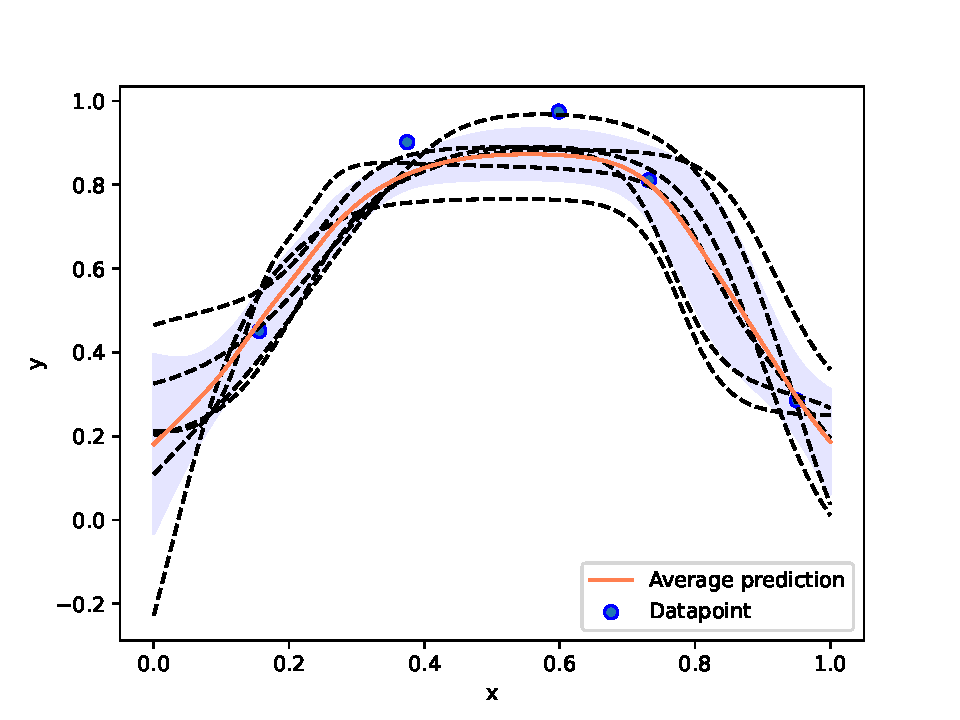
\includegraphics[width=\textwidth,height=\textheight,keepaspectratio]{pics/figure_simple_BNN.pdf}
    \caption{Sampled neural networks from a predictive posterior that is based on a Gaussian prior and a Gaussian likelihood on the 6 datapoints. The average prediction of the networks are plotted along with a filled area defined by the average plus minus the standard deviation of the network predictions to represent uncertainty. \textcolor{red}{Include and refer to code in appendix.}}
    \label{fig:simple_BNN}
\end{figure}

\noindent
A simple example, inspired by \cite{neal2012bayesian}, will illustrate the general concept of Bayesian learning for neural networks and the inefficiency of brute force methods. Figure \ref{fig:simple_BNN} shows 6 BNNs whose weights and biases were drawn from independent standard normal prior distributions except output weights, which had a standard deviation of $\frac{1}{\sqrt{16}}$. The networks performs regression on 6 datapoints for which the prior and the likelihood was based. \\
\\
The 6 networks was chosen from a larger pool of $10^5$ networks whose weights and biases were sampled from identical prior distributions. The likelihood was computed for each of these networks and scaled so that the largest likelihood was 1. The networks were then accepted with the probability of this scaled likelihood for which only 6 was accepted. This approach resembles rejection sampling and embodies the posterior in \ref{eq:posterior} by making the prior control the generation of candidate networks and the likelihood control which of these candidates are rejected.\\
\\
We follow the suggestion of \cite{neal2012bayesian} to model regression tasks with a conditional distribution for the real valued targets $\boldsymbol{y}_k$, from $k$ neural networks with outputs $f_k(\boldsymbol{x})$, defined by a Gaussian 
\begin{equation}\label{eq:regr_taget_distribution}
    p(\boldsymbol{y} \mid \boldsymbol{x}) = \prod_k \frac{1}{\sqrt{2 \pi} \sigma_k} \exp{- \frac{\lr{f_k(\boldsymbol{x}) - y_k}^2}{2 \sigma_k^2}}
\end{equation}
with mean $f_k(x)$ and standard deviation $\sigma_k$ as a hyperparameter, which we chose to be $\sigma_k = 0.1$ for all $k$.
\\
\\
The optimal way to predict the target associated with various new examples, assuming we want to minimize the expected squared error, is to predict the mean of the predictive distribution in equation \ref{eq:post_pred_distribution}. For a regression model defined by equation \ref{eq:regr_taget_distribution} this is equal to predicting 
\begin{equation*}
    \hat{\boldsymbol{y}}^{(n+1)} = \int f\lr{\boldsymbol{x}^{(n+1)}, \boldsymbol{\theta}} p\lr{\boldsymbol{\theta} \mid \lr{\boldsymbol{x}^{(1)}, \boldsymbol{y}^{(1)}}, \dots, \lr{\boldsymbol{x}^{(n+1)}, \boldsymbol{y}^{(n+1)}}} \, d \boldsymbol{\theta}
\end{equation*}
As we can only sample from this distribution we resort to a Monte Carlo approximation by averaging over the 6 functions drawn from the posterior as in equation \ref{eq:empirical_mean_MC}. This is also equivalent to minimizing mean squared error. The average is shown in \ref{fig:simple_BNN} by the dotted line. But Bayesian inference can do more than a single-valued guess. By examining the function we can also see the uncertainty of the guesses, for example how rapidly uncertainty increases beyond the region of the datapoints. 
\\
\\
This shows some of the perks of using Bayesian inference for neural networks, but what remains is the downside of computational time. Generating $10^5$ samples to get 6 draws from the posterior not very efficient and this only becomes more infeasible as the number of datapoints increase. In section \ref{sec:MCMC} we discuss how to sample more effectively from the posterior using Markov-Chain Monte Carlo methods. Another unresolved matter is how to choose the prior, and how this choice affects our results. This is discussed in section \ref{sec:priors} while how to efficiently choose the parameters of the prior using a distribution is discussed in section \ref{sec:hier_models}.



\section{Markov Chain Monte Carlo}\label{sec:MCMC}
 As mentioned in section \ref{sec:bayesian_stat} the posterior distribution is often intractable and we might need simulation based methods to find a feasible solution. We want to be able to calculate posterior summaries like $\mathbb{E}_{\hat{p}}\left[f(\boldsymbol{\theta})\right]$ where $f(\boldsymbol{\theta})$ is some function and the expectation is taking under the posterior distribution. Such an expectation is straightforward to approximate using the simple Monte Carlo methods, described in section \ref{sec:MC_methods}, when dealing with nice and low dimensional distributions. Other Methods like importance sampling has often been proposed in the litterateur for simple problems, but rarely for high-dimensional problems as we often face with Neural Networks.
 \\
 \\
As demonstrated in section \ref{sec:simple_BNN} simple sample methods like the ones in section \ref{sec:MC_methods} are not very useful in complex models like BNNs and we are instead motivated to use a collection of more sophisticated methods. This dissertation will mainly pursue this motivation by exploring the Markov chain Monte Carlo (MCMC) methods. The main idea of these is to simulate a Markov chain, which has the posterior distribution as its stationary distribution. We will initially give a concise explanation of the fundamentals of Markov Chains in section \ref{sec:basic_mc} and follow this by exploring the most popular MCMC-algorithms for sampling in BNNs.
A deeper discussion of Markov chains than provided in this dissertation can be found in \cite{lawler2006introduction}.
 
\subsection{Markov Chains}\label{sec:basic_mc}

A stochastic process is a set of random variables that are defined over some probability space $\left\{X^{(t)} \right\}_{t\in T}$, where $T\subset \mathbb{R}$ is the indexation and may be considered as a temporal or a time index. In the context of Machine Learning, the set $T$ can be interpreted as the iterations of a simulation scheme. In stochastic simulation we typically have that $T=\mathbb{N}$ and we can write the stochastic process as $\left\{X^{(n)}\right\}_{n\geq 0}$, where $n$ reminds us that we have discrete index set. Throughout this thesis we will only consider discrete time stochastic processes, since this is most relevant when discussing stochastic simulation. \\
The state space is the set of the process $\left\{X^{(n)} \right\}_{n\geq 0}$, and will in most application by either integers or real values and is denoted by $\mathbb{S}$. 
\\
\\
As in section \ref{sec:simple_BNN} we want to sample from the posterior predictive distribution, that's likely intractable, and we do this by trying to sample from the posterior of the weights and send these sampled weights through the network to obtain network-outputs, that are then used to find samples from the posterior predictive distribution. This shows how we consider the model parameters $\boldsymbol{\theta}$ as random variables and aims to sample from the posterior of these. To do this using MCMC we can consider the stochastic process $\{\boldsymbol{\theta}^{(n)}\}_{n\geq 0}$. We call the distribution we wish to sample from the target distribution and denote it $\hat{p}(\cdot)$. The target distribution in case of BNNs is the posterior of the weights so that $\hat{p}(\boldsymbol{\theta})\equiv p(\boldsymbol{\theta}\mid \mathbf{X},\mathbf{y})$.
\\
\\
Using Markov Chain Monte Carlo we aim to sample from a stochastic process satisfying the Markov property. Such a process is defined by being dependant only on the previous state of the process and a set of transitional probabilities and is called a Markov chain. The Markov chain is defined by an initial distribution for the first state of the chain $\boldsymbol{\theta}^{(0)}$, and transition probability or density for continuous state processes, for the next states in the system. We write the transition density from transitioning from state $\boldsymbol{\theta}^{(n-1)}$ to another state $\boldsymbol{\theta}^{(n)}$ as $T(\boldsymbol{\theta}^{(n)}\mid \boldsymbol{\theta}^{(n-1)})$. \\
\\
When sampling from the Markov chain we want to make sure that samples are actually coming from the desired distribution $\hat{p}(\boldsymbol{\theta})$ no matter the initial probability. To ensure this we must generate a Markov chain that has a stationary distribution that is our desired distribution $\hat{p}\lr{\boldsymbol{\theta}}$. That is if $\boldsymbol{\theta}^{(n-1)}$ has distribution $\hat{p}(\boldsymbol{\theta})$, then  $\boldsymbol{\theta}^{(n)}$ will have the same distribution, and this will hold for all future states of the chain. The property of a Markov chain having a stationary distribution is called the invariance property and is defined by
\begin{equation*}
    \pi(\boldsymbol{\theta}^{(n)})=\int T(\boldsymbol{\theta}^{(n)}\mid \boldsymbol{\theta}) \pi(\boldsymbol{\theta})d\boldsymbol{\theta}
\end{equation*}
A sufficient, but not necessary condition that ensures that a particular $\hat{p}(\boldsymbol{\theta})$ is stationary distribution is the detailed balance condition. The condition states if we let $T(\cdot,\cdot)$ be a transition density, which satisfies the following condition $T(\boldsymbol{\theta}^{(n-1)}, \boldsymbol{\theta}^{(n)}) \hat{p}(\boldsymbol{\theta}^{(n)})= T(\boldsymbol{\theta}^{(n)}, \boldsymbol{\theta}^{(n-1)})\hat{p}(\boldsymbol{\theta}^{(n-1)})$, then $\hat{p}(\cdot)$ is a stationary distribution of the Markov chain associated with the transition density $T(\cdot,\cdot)$. This property however only ensures that $\hat{p}\lr{\boldsymbol{\theta}}$ is stationary distribution and not that it is the only one, meaning that our Markov chain can end up sampling from the wrong distribution even though it satisfies the detailed balance condition.
\\
\\
To guarantee that we sample from $\hat{p} \lr{\boldsymbol{\theta}}$ we need to ensure that the Markov chain only has this distribution as a stationary distribution. A Markov chain which has a unique stationary distribution from which it converges to from any initial state is called an ergodic Markov chain (see e.g \cite{turkman2019computational}). For a Markov chain to be ergodic, it needs to satisfy two conditions for the states of the system and the transition densities. These conditions are known as irreducibility and aperiodicity. 
\\
\\
Often we discard or burn some of the initial states, since these may not be representative of the desired distribution as the chain might not have reached the stationary distribution yet. These discarded steps are part of what is called the  burn-in period of the Markov chain. When the chain has reached the stationary distribution, it is possible to draw as many identical distributed samples as we wish for, but one should note that any successive samples will be highly correlated with each other and therefore not necessarily a good representative for the target distribution. \cite{Goodfellow-et-al-2016} suggest a way to come around this problem, by only returning every $n$ successive sample. Because of both the burn-in period and the time required for the chain to return uncorrelated samples MCMCs are often computational expensive. \\
\\
In order to produce truly independent samples, \cite{Goodfellow-et-al-2016} suggest to run multiple Markov chains in parallel. They also mention that practitioners often chooses the number of chains to run in parallel, similar to the number of examples in a mini-batch and then draw the samples needed from this set of Markov chains. 


\subsection{The Metropolis Algorithm} \label{sec:Metropolis}
The Metropolis algorithm is a Markov chain Monte Carlo (MCMC) method, which is used to sample from a Bayesian posterior. 
The Metropolis algorithm was originally introduced by \cite{Metropolis1953} and was developed to simulate the states for a system of idealized molecules (\cite{neal2012mcmc}). This was later further developed by \cite{hastings70}, so that the algorithm could now simulate from a general distribution and not just a symmetric one, as it was previously based on. Due to its versatility and simplicity, the Metropolis algorithm is one of the most widely used MCMC method.\\
\\
The Metropolis algorithm generates a sequence of stochastic variables by sampling from a probability distribution, more specific the samples are drawn from a proposal distribution, that specifies the probability of moving to a new point in the sample space. \\
As mentioned in section \ref{sec:MCMC}, the main idea is to create a Markov chain that will converge towards a given distribution, so that the target distribution becomes the Markov chain's stationary distribution.  \\
\\
The simple Metropolis algorithm introduced in the original paper by \cite{Metropolis1953} consider a target distribution $\hat{p}(\boldsymbol{\theta})$ and a proposal distribution $q(\boldsymbol{\theta})$. The algorithm generates a Markov chain, by starting the chain at some arbitrarily point generated from the proposal distribution $\boldsymbol{\theta}^{(0)}\sim q(\boldsymbol{\theta})$ and then proposing a candidate state for the next state in the chain $\boldsymbol{\theta}^{\text{\text{cand}}}$, where this candidate state is drawn from the conditional distribution on the previous state $\boldsymbol{\theta}^{\text{\text{cand}}}\sim q(\boldsymbol{\theta}^{(n+1)}\mid\boldsymbol{\theta}^{(n)})$. We then decide whether or not to reject this new state based on the relative density to the old state. If the relative density is larger than one, we accept the new state, if the relative density is less than one, we accept the new state with probability $\frac{\hat{p}(\boldsymbol{\theta}^{\text{\text{cand}}})}{\hat{p}(\boldsymbol{\theta}^{(n)})}$. In this context the Metropolis algorithm imposes the symmetry condition of on the proposal distribution, so that
\begin{equation*}
    q(\boldsymbol{\theta}^{(n)}\mid \boldsymbol{\theta}^{(n-1)})=q(\boldsymbol{\theta}^{(n-1)}\mid \boldsymbol{\theta}^{(n)})
\end{equation*}
A pseudo code version of the Metropolis algorithm can be seen in algorithm \ref{algo_2}.
% Metropolis Algorithm
\begin{algorithm}\label{algo_2}

\SetAlgoLined
initialize $\boldsymbol{\theta}^{(0)}\sim q(\boldsymbol{\theta})$;

\For{$n=1,2,\ldots$}{
Propose: $\boldsymbol{\theta}^{\text{\text{cand}}} \sim q\left(\boldsymbol{\theta}^{(n)} \mid \boldsymbol{\theta}^{(n-1)}\right)$

Acceptance Probability:

$ \alpha\left(\boldsymbol{\theta}^{\text{\text{cand}}} \mid \boldsymbol{\theta}^{(n-1)}\right)=\min \left\{1, \frac{\hat{p}\left(\boldsymbol{\theta}^{\text{\text{cand}}}\right)}{ \hat{p}\left(\boldsymbol{\theta}^{(n-1)}\right)}\right\} $

$u \sim  \text { Uniform }(0,1)
$

  \uIf{$u<\alpha$}{
    Accept the proposal: $\boldsymbol{\theta}^{(n)} \leftarrow \boldsymbol{\theta}^{\text{\text{cand}}}$\;
  }
  \Else{
    Reject the proposal: $\boldsymbol{\theta}^{(n)} \leftarrow \boldsymbol{\theta}^{(n-1)}$ \;
  }
    }
\caption{Metropolis algorithm \textcolor{red}{Edit with input and output description.}}
\end{algorithm}\\
One apparent problem is that we don't know the posterior, which is our target distribution $\hat{p}\lr{\boldsymbol{\theta}}$, so we can't directly calculate $\frac{\hat{p}(\boldsymbol{\theta}^{(n)})}{\hat{p}\left(\boldsymbol{\theta}^{(n-1)}\right)}$. But since the algorithm only need the target distribution for calculating this relative density, we can use equation \ref{eq:posterior} and calculate the ratio of the likelihood times the prior. 
\\
\\
To show that the Metropolis algorithm is in fact sampling from the target distribution, we must show that the Markov chain converges to a stationary distribution which is our target distribution. If we assume that the Markov Chain is ergodic we can do this by showing that the metropolis satisfies the detailed balanced condition explained in section \ref{sec:MCMC}.\\
\\
For $\boldsymbol{\theta}^{(n)}\neq \boldsymbol{\theta}^{(n-1)}$ the Metropolis algorithm has the following transitions densities,
\begin{equation*}
    T\left(\boldsymbol{\theta}^{(n)} \mid \boldsymbol{\theta}^{(n-1)}\right)=q\left(\boldsymbol{\theta}^{(n)} \mid \boldsymbol{\theta}^{(n-1)}\right) \min \left(1, \frac{\hat{p}\left(\boldsymbol{\theta}^{(n)}\right)}{ \hat{p}(\boldsymbol{\theta}^{(n-1)})}\right)
\end{equation*}
We can show that this satisfies the detailed balanced condition by
\begin{equation*}
\begin{aligned}
T\left(\boldsymbol{\theta}^{(n)} \mid \boldsymbol{\theta}^{(n-1)}\right) \hat{p}(\boldsymbol{\theta}^{(n-1)}) &=q\left(\boldsymbol{\theta}^{(n)} \mid \boldsymbol{\theta}^{(n-1)}\right) \min \left(1,\frac{ \hat{p}\left(\boldsymbol{\theta}^{(n)}\right) }{ \hat{p}(\boldsymbol{\theta}^{(n-1)})}\right) \hat{p}(\boldsymbol{\theta}^{(n-1)}) \\
&=q\left(\boldsymbol{\theta}^{(n)} \mid \boldsymbol{\theta}^{(n-1)}\right) \min \left(\hat{p}(\boldsymbol{\theta}^{(n-1)}), \hat{p}\left(\boldsymbol{\theta}^{(n)}\right)\right) \\
&=q\left(\boldsymbol{\theta}^{(n-1)} \mid \boldsymbol{\theta}^{(n)}\right) \min \left(\hat{p}\left(\boldsymbol{\theta}^{(n-1)}\right), \hat{p}(\boldsymbol{\theta}^{(n-1)})\right) \\
&=q\left(\boldsymbol{\theta}^{(n-1)} \mid \boldsymbol{\theta}^{(n)}\right) \min \left(1, \frac{\hat{p}(\boldsymbol{\theta}^{(n-1)}) }{ \hat{p}\left(\boldsymbol{\theta}^{(n)}\right)}\right) \hat{p}\left(\boldsymbol{\theta}^{(n)}\right) \\
&=T\left(\boldsymbol{\theta}^{(n-1)} \mid \boldsymbol{\theta}^{(n)}\right) \hat{p}\left(\boldsymbol{\theta}^{(n)}\right)
\end{aligned}
\end{equation*}
This shows that the transitions proposed by the algorithm leaves the target distribution $\hat{p}(\boldsymbol{\theta})$ invariant and therefore samples produced by this Markov chain all has the same stationary distribution $\hat{p}(\boldsymbol{\theta})$, provided that the Markov chain is ergodic. However according to \cite{neal2012bayesian} the Metropolis algorithm will not always produce an ergodic Markov chain and that this depends on the details of the target distribution and proposal distribution. If the produced Markov chain is not ergodic we might end up sampling from a stationary distribution that is not our target distribution.
\\
\\
Many choices are possible for the proposal distribution. \cite{neal2012bayesian} mentions that a simple choice could be a Gaussian centered on $\boldsymbol{\theta}^{(n)}$ with standard deviation chosen to that acceptance probability of the candidate state is reasonably high, since a very low acceptance ratio is usually bad, as the successive states will be highly dependant. He also notes that when sampling from high-dimensional and complex distributions, as is often the case with posteriors in BNNs, the standard deviation of such a proposal distribution will often have to be small compared to the extent of the target distribution, as large changes almost certainly will lead to a region of low probability. This will result in highly dependant states and many steps will be needed to arrive at distant points in the distribution. \cite{gelmanbda04} suggests coping with this problem by throwing away some of the samples or run multiple chains in parallel. \\
\\
\cite{neal2012bayesian} further mentions that this problem with Metropolis is made worse due to its movements taking the inefficient form of a random walk instead of a systematic path, as can be seen in the illustration of a sampling with Metropolis in figure \ref{fig:MH_sampling}. This inefficient movement yields slower convergence to the target distribution. This drawback, will be even more prominent in higher dimension and for more complex target distributions according to \cite{gelmanbda04}. \\
\\
A more generalized version of the algorithm is the one introduced by \cite{hastings70}, which allows for non-symmetric proposal distributions, that is $q(\boldsymbol{\theta}^{(n)}\mid \boldsymbol{\theta}^{(n-1)}) \neq q(\boldsymbol{\theta}^{(n-1)}\mid \boldsymbol{\theta}^{(n)})$. To correct for this asymmetry in the proposal distribution, the acceptance ratio is replaced by
\begin{equation}\label{eq: hasti_pasti}
\alpha\left(\boldsymbol{\theta}^{c a n d} \mid \boldsymbol{\theta}^{(n-1)}\right)=\min \left\{1, \frac{q\left(\boldsymbol{\theta}^{(n-1)} \mid \boldsymbol{\theta}^{c a n d}\right) \hat{p}\left(\boldsymbol{\theta}^{c a n d}\right)}{q\left(\boldsymbol{\theta}^{c a n d} \mid \boldsymbol{\theta}^{(n-1)}\right) \hat{p}\left(\boldsymbol{\theta}^{(n-1)}\right)}\right\} 
\end{equation}
One should note that the Metropolis algorithm is an instance of the generalized version, since equation \ref{eq: hasti_pasti} is identical to the acceptance ratio in the original algorithm when allowance for a symmetric distribution. \\
\\
The introduction of an asymmetric proposal distribution, is often useful when we want to increase the speed of the random walk generated by Metropolis algorithm, but this is often not sufficient for complicated models with high-dimensional target distributions as we face with Bayesian Neural Networks (\cite{gelmanbda04}). We will in the next chapter concentrate on a more efficient way of simulating the chain.
\begin{figure}
    \centering
    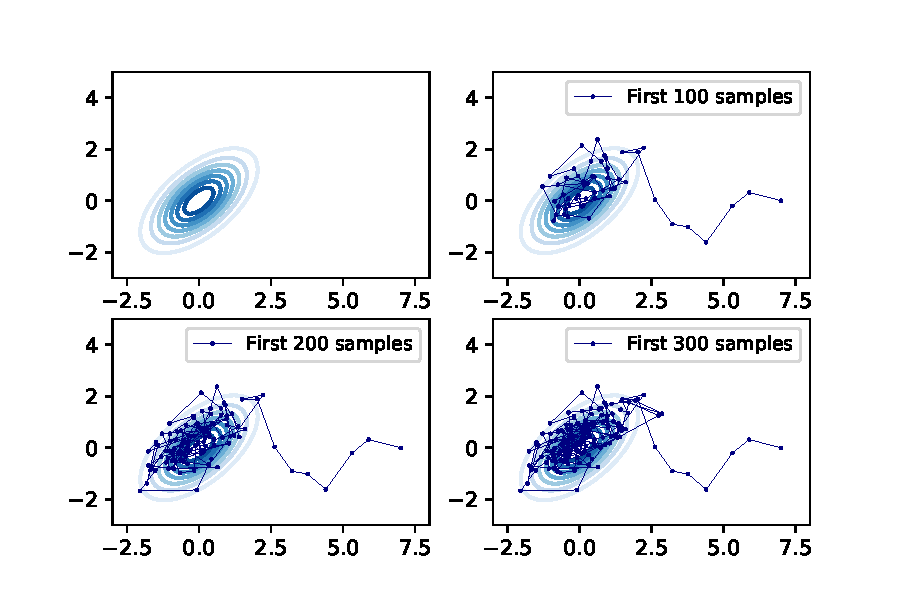
\includegraphics[width=\textwidth, height=\textheight, keepaspectratio]{pics/mh_randomWalk_behavior.pdf}
    \caption{Illustration of the convergence to a target distribution with 300 samples from the Metropolis algorithm. The target distribution is a bivariate Gaussian with mean 
        $\boldsymbol{\mu}= \begin{bmatrix}
            0 & 0
            \end{bmatrix}$ and covariance matrix
            $\boldsymbol{\Sigma}= 
            \begin{bmatrix}
                1 & 0.6\\
                0.6 & 1   
            \end{bmatrix}$. The Python code for producing this figure can be found in appendix \ref{app:MH_code}.
    }
    \label{fig:MH_sampling}
\end{figure}
\clearpage

\section{Hamiltonian Monte Carlo}
Another way to generate proposals with a higher efficiency, is by updating the parameters by dynamical simulation and then use the Metropolis algorithm to accept or reject these proposals. Such an algorithm suppress the local random walk behavior and allows it to move faster and more rapidly through the target distribution. This method, which, we will present in this chapter, is called Hamiltonian Monte Carlo (HMC), and is commonly used in computational physics and statistics. The algorithm was originally proposed by \cite{Duane1987216} for calculations used in lattice quantum chromodynamics, but was later introduced to the field of computational statistics when it was used for Bayesian Neural Networks in \cite{neal2012bayesian}. This means that the Markov Chain from which we sample in BNNs is produced analogous to paths of particles using Hamiltonian dynamics, and we will explain these dynamics using this physical analogy, as it gives a more intuitive idea of HMC.
\\
\\
It turns out that the HMC algorithm reduces correlation between successive sampled states, compared to the Metropolis Hastings algorithm in section \ref{sec:Metropolis}, by proposing moves to distant states of the target distribution, which maintain a high probability of acceptance due to the properties of the simulated Hamiltonian dynamics. The reduced correlation means fewer Markov chain samples are needed to approximate integrals with respect to the target probability distribution.

\subsection{Hamiltonian Dynamics}
Before we move to the actual HMC algorithm, we will explain the Hamiltonian dynamics from which we produce the Markov chain for the algorithm. The Hamiltonian dynamics are used to describe how an object move around in a system or space. It is defined by the objects position $\boldsymbol{q}\in \mathbb{R}^d$ and its momentum $\boldsymbol{\rho}\in \mathbb{R}^d$, which in the field of physics are equivalent to an object's mass times its velocity at some point in time. When performing HMC to generate samples from the target distribution $\hat{p}(\boldsymbol{\theta})$, the position variable plays the role as the parameter vector and for now on we will let $\boldsymbol{\theta}:=\boldsymbol{q}$. The object's position is associated with a potential energy $U(\boldsymbol{\theta})$ and likewise the momentum is associated with a kinetic energy $K(\boldsymbol{\rho})$. The sum of the potential and kinetic energy is regarded as the total energy of the system and often called the Hamiltonian
\begin{equation*}
H(\boldsymbol{\theta},\boldsymbol{\rho})=U(\boldsymbol{\theta})+K(\boldsymbol{\rho})    
\end{equation*}       
one important feature of the Hamiltonian is that it is constant over time. Taking the partial derivative with respect to time of the position and momentum, shows us how they evolve over time
\begin{equation}\label{eq:hamilton_equations}
\begin{split}
\frac{d \theta_{i}}{d t}=\frac{\partial H}{\partial \rho_{i}}=\frac{\partial K(\boldsymbol{\rho})}{\partial \rho_{i}} \\
\frac{d \rho_{i}}{d t}=-\frac{\partial H}{\partial \theta_{i}}=-\frac{\partial U(\boldsymbol{\theta})}{\partial \theta_{i}}
\end{split}
\end{equation}
where $i=1,2, \ldots,d$. These are named Hamiltonian equations and represents a differential equations system. The Hamiltonian equations are very useful, since if we are able to evaluate the partial derivatives from equation \ref{eq:hamilton_equations}, we are able to predict the position and momentum variable of the object at any point in the future $t^\prime>t$. \cite{neal2012bayesian} shows that these dynamics along with the energy conserving property of the Hamiltonian results in the process being reversible and preserving of volume of the phase space, which in turn provides a stationary distribution. 


\subsection{Discretizing Hamiltonian Equations}
The Hamiltonian equations describe how an objective evolve in continuous time, but for simulating Hamiltonian dynamics on a computer system, we have to approximate the differential equations numerically in some way, this is done by discretizing time. We do this by splitting the time interval $dt$ into small intervals $\varepsilon$. 
\\
\\
The usual discretizing scheme for simulating Hamiltonian equations, is the Leapfrog method. The Leapfrog method takes a half step to update momentum variable then a whole step to update the position value, and finally the last half step to update momentum
\begin{equation*}
\begin{split}
\rho_{i}^{(t+\varepsilon / 2)}=\rho_{i}^{(t)}-(\varepsilon / 2) \frac{\partial U}{\partial \theta_{i}^{(t)}} \\
\theta_{i}^{(t+\varepsilon)}=\theta_{i}^{(t)}+\varepsilon \frac{\partial K}{\partial \rho_{i}^{(t+\varepsilon / 2)}} \\
\rho_{i}^{(t+\varepsilon)}=\rho_{i}^{(t)}-(\varepsilon / 2) \frac{\partial U}{\partial \theta_{i}^{(t+\varepsilon)}}
\end{split}
\end{equation*}
According to \cite{neal2012mcmc} the Leapfrog preserves the HMC properties of being reversible and preserve volume of the phase space, ensuring that we sample a stationary distribution.


\subsection{Hamiltonian and Probability: Canonical Distributions}
We have now explained what a Hamiltonian is and how we can simulate its dynamics by using the Leapfrog method. We will now connect this to MCMC theory from the previous sections in order to explain how to use HMC to sample from the posterior of the weights in a BNN. In order to perform this connection, we need to relate the target distribution and the Hamiltonian, such that we can use the Hamiltonian equations to sample from the target distribution. A way of doing this, proposed by \cite{neal2012bayesian}, is to use a concept from statistical mechanics known as the canonical (Boltzmann) distribution. We can write a probability distribution on $\boldsymbol{\theta}$ under the canonical distribution as
\begin{equation*}
    p(\boldsymbol{\theta})\propto \exp\left(\frac{-E(\boldsymbol{\theta})}{T}\right)
\end{equation*}
where $E(\boldsymbol{\theta})$ can be any energy function defined over $\boldsymbol{\theta}$. $T$ is often called the temperature of the system and usually chosen to be equal to one as it plays no role in this application (\cite{neal2012bayesian}).
One should note that any probability distribution that is nowhere zero can be put into this form by letting $E(\boldsymbol{\theta})=-\log p(\boldsymbol{\theta})-\log Z$, for any convenient choice of normalization constant $Z$. Since the Hamiltonian is an energy function for the joint state of both position and momentum, a joint distribution can be defined by
\begin{equation*}
p(\boldsymbol{\theta},\boldsymbol{\rho})\propto \exp(-\H(\boldsymbol{\theta},\boldsymbol{\rho}))   = \exp(-U(\boldsymbol{\theta}))\exp(-K(\boldsymbol{\rho}))
\end{equation*}
Assuming Independence between $\boldsymbol{\theta}$ and $\boldsymbol{\rho}$ we can by the equation above write $U(\boldsymbol{\theta})=-\log p(\boldsymbol{\theta})$ and $K(\boldsymbol{\rho})=-\log p(\boldsymbol{\rho})$ meaning that the Hamiltonian can be interpreted as the log joint distribution on $(\boldsymbol{\theta},\boldsymbol{\rho})$. 
\\
\\
We now have a joint distribution, in terms of the Hamiltonian function, which we know how to sample from. But we are in fact only interested in samples of the position variable $\boldsymbol{\theta}$, which is samples from our target distribution. Meanwhile we are not interested in the momentum variable $\boldsymbol{\rho}$, which is only introduced to make the algorithm move faster through the parameter space. This means that we can chose the marginal distribution of momentum arbitrarily. This is often chosen by practitioners to be Gaussian, $\boldsymbol{\rho}\sim \mathcal{N}\left(0, \Sigma \right)$, where $\Sigma$ is some symmetric, positive-definite covariance matrix and often chosen to be diagonal, such that $\boldsymbol{\rho}$ is $d$-dimensional multivariate Gaussian, with the $d$ variables being independent. We follow the simple approach from \cite{hoffman2011nouturn} and let $\mathbf{\Sigma}$ be the identity matrix $\mathit{I}$. This makes the dynamics of equation \ref{eq:hamilton_equations} simplify to 
\begin{equation*}
\begin{split}
\frac{d \theta_{i}}{d t}&=\rho_i \\
\frac{d \rho_{i}}{d t}&=\frac{\partial \log p(\theta_{i})}{\partial \theta_i} 
\end{split}
\end{equation*}
A more rigorous examination of possible choices for the covariance matrices is provided by \cite{neal2012mcmc}. 



\subsection{Hamiltonian Monte Carlo}
We start the HMC algorithm from an initial state $\boldsymbol{\theta}^{(0)}$ $\boldsymbol{\rho}^{(0)}$, and then we simulate the Hamiltonian dynamics for $t+\varepsilon$ using the Leapfrog method. The states generated for the position and momentum variable at the end of the Leapfrog simulation is used as proposals for a new state $(\boldsymbol{\theta}^{\text{cand}},\boldsymbol{\rho}^{\text{cand}})$. These samples need to be proposed and accepted according to a criteria, because the leapfrog-discretization provides an error term in its approximation of the continuous Hamiltonian dynamics. This criteria is the Metropolis acceptance criteria,
\begin{equation}\label{eq:hmc_acceptance}
\begin{split}
    \alpha\left((\boldsymbol{\theta},\boldsymbol{\rho}) \mapsto (\boldsymbol{\theta}^{\text{cand}} , \boldsymbol{\rho}^{\text{cand}} )\right) &= \min\left\{1, \frac{p(\boldsymbol{\theta}^{\text{cand}},\boldsymbol{\rho}^{\text{cand}})}{p(\boldsymbol{\theta},\boldsymbol{\rho})} \right\}\\
    &= \min\{1,\exp\left(\log p(\boldsymbol{\theta}^{\text{cand}},\boldsymbol{\rho}^{\text{cand}})- \log p(\boldsymbol{\theta}, \boldsymbol{\rho})  \right)\\
    &= \min \left\{1,\exp\left(-\H(\boldsymbol{\theta}^{\text{cand}},\boldsymbol{\rho}^{\text{cand}}) +\H(\boldsymbol{\theta},\boldsymbol{\rho})\right) \right\}
\end{split}
\end{equation}
This means that we do as in the metropolis algorithm, but using distributions provided by the Hamiltonian dynamics. With $\boldsymbol{\rho}\sim \mathcal{N}\left(0,\mathit{I}\right)$ this is equivalent to
\begin{equation*}
\alpha\left((\boldsymbol{\theta},\boldsymbol{\rho}) \mapsto (\boldsymbol{\theta}^{\text{cand}} , \boldsymbol{\rho}^{\text{cand}} )\right) 
=\min\left\{1,\frac{\exp\left(\mathcal{L}(\boldsymbol{\theta}^{\text{cand}})-\frac{1}{2}\boldsymbol{\rho}^{\text{(cand)}^\top}\boldsymbol{\rho}^{\text{(cand)}}\right)}{\exp\left(\mathcal{L}(\boldsymbol{\theta})-\frac{1}{2}\boldsymbol{\rho}^\top\boldsymbol{\rho}\right)}\right\}
\end{equation*}
where $\mathcal{L}\left(\boldsymbol{\theta}\right)$ is the log-probability distribution on $\boldsymbol{\theta}$.
\\ 
\\
We see from the last part in equation \ref{eq:hmc_acceptance}, that if we could perfectly discretize the Hamiltonian dynamics the Metropolis acceptance criteria would always be equal to one, due to the Hamiltonian conservation criteria (see e.g \cite{neal2012mcmc}), but since we usually can't, it will often be lower. We can see that if we get a small error in the discretization the term  $\H(\boldsymbol{\theta},\boldsymbol{\rho})-\H(\boldsymbol{\theta}^{\text{cand}},\boldsymbol{\rho}^{\text{cand}})$ in the exponent should be small, yielding a high acceptance rate. This way of making proposals is beneficial since it allows the Markov Chain to effectively make very large and uncorrelated moves in the state space, while keeping a high acceptance of probability. HMC is written in pseudo code in algorithm \ref{alg:HMC}. It takes in an initial value for the parameters $\boldsymbol{\theta}^{(0)}$ which is the starting point of the algorithm. The input $\mathcal{L}$ is the log-probability distribution of $\boldsymbol{\theta}$, which is defined to be equal to the negative potential energy function. In BNN this is identical to the log-posterior distribution on the network parameters. One need to be able to at least evaluate the posterior distribution and its gradient or alternatively something proportional to it. In our case where the target distribution is the posterior distribution, we know that it is proportional to the likelihood and the prior, which we in most cases are able to evaluate. The $M$ input is the number of total iterations one would like to perform.
\\
\\
The algorithm also relies on a stepsize $\varepsilon$ variable, that defines the size of the leapfrog step. If $\varepsilon$ is chosen too be to large, the the Leapfrog simulation of the Hamiltonian will be inaccurate and lead to a very low rate of acceptance making the algorithm ineffectively waste computational time. On the other hand, if we choose $\varepsilon$ to be too small, we will waste computational time by taking too small steps. The sampling is also affected by a hyperparameter $L$, that defines how many Leapfrog steps the algorithm performs before proposing a new candidate state. A too small value for $L$ will give successive samples that lies close to each other which results in the same undesirable random walk behavior as the Metropolis algorithm from section \ref{sec:Metropolis}. Too large a value for $L$ might produce inaccurate samples and can produce trajectories that loops back and retrace their steps, a behavior called U-turns. Tuning these parameters can be hard and we are often forced to rely on heuristics based on autocorrelation statistics from preliminary runs (\cite{neal2012mcmc}).
\\
\\
In figure \ref{fig:HMC_Example} we have illustrated how HMC propose a candidate sample for a bivariate $\mathcal{N}\left(\mathbf{0},\mathit{I}\right)$ target distribution. In subfigure (a) and (b) we have chosen a proper value for $\varepsilon$ and $L$ such that the algorithm generates proposals that are appropriately far from the previous ones. In subfigure (c) and (d) we have chosen larger values for $\varepsilon$ and $L$, and we can see that the algorithm starts too loop-back, which results in identical proposals for each iteration and a large proportion of the target distribution will therefore never be visited. In the next section we will look into a modification of the HMC algorithm, such that we can avoid this kind of U-turn behavior.  


\begin{algorithm}\label{alg:HMC}
\SetAlgoLined
\SetKwFunction{Leapfrog}{Leapfrog}
$\text{Given } \boldsymbol{\theta}^{(0)},  \mathcal{L}, M, \varepsilon, L,$:\\
\For{m=1 to M}{
Sample $\boldsymbol{\rho}^{(0)} \sim \mathcal{N}(0, \mathbf{\mathit{I}})$ \\
Set $ \boldsymbol{\theta}^{\text{cand}} \leftarrow \boldsymbol{\theta}^{(m-1)}, \boldsymbol{\rho}^{\text{cand}} \leftarrow \boldsymbol{\rho}^{(0)}$\\
\For{i = 1 to L}{
Set $\boldsymbol{\theta}^{\text{cand}}, \boldsymbol{\rho}^{\text{cand}} \leftarrow \Leapfrog(\boldsymbol{\theta}^{\text{cand}}, \boldsymbol{\rho}^{\text{cand}}, \varepsilon)$
}
Negate momentum: $\boldsymbol{\rho}^{\text{cand}} \leftarrow - \boldsymbol{\rho}^{\text{cand}}$\\
Compute acceptance probability:\\
$\alpha=\min \left\{1, \frac{\exp \left\{\mathcal{L}(\boldsymbol{\theta}^{\text{cand}})-\frac{1}{2} \boldsymbol{\rho}^{\text{(cand)}^\top}  \boldsymbol{\rho}^{\text{cand}}\right\}}{\exp \left\{\mathcal{L}\left(\boldsymbol{\theta}^{(m-1)}\right)-\frac{1}{2} \boldsymbol{\rho}^{(0)^\top}  \boldsymbol{\rho}^{(0)}\right\}}\right\}$\\
Sample $u\sim \text{Uniform}(0,1)$\\
 \uIf{$u<\alpha$}{
    Accept the proposal: $\boldsymbol{\theta}^{(m)} \leftarrow \boldsymbol{\theta}^{c a n d}$\;
  }
  \Else{
    Reject the proposal: $\boldsymbol{\theta}^{(m)} \leftarrow \boldsymbol{\theta}^{(m-1)}$ \;
  }
}
\SetKwProg{Fn}{Function}{:}{\KwRet{$\boldsymbol{\theta}^{\text{cand}},\boldsymbol{\rho}^{\text{cand}}$}}
\Fn{\Leapfrog{$\boldsymbol{\theta}$, $\boldsymbol{\rho}$, $\varepsilon$}}{
 Set $\boldsymbol{\rho}^{\text{cand}} \leftarrow \boldsymbol{\rho}^{\text{cand}}+(\varepsilon / 2) \nabla_{\theta} \mathcal{L}(\theta)$\\
Set $\boldsymbol{\theta}^{\text{cand}} \leftarrow \theta+\varepsilon \boldsymbol{\rho}^{\text{cand}}$\\
Set  $\boldsymbol{\rho}^{\text{cand}} \leftarrow \boldsymbol{\rho}
^{\text{cand}}+(\varepsilon / 2) \nabla_{\theta} \mathcal{L}(\boldsymbol{\theta}^{\text{cand}})$
  }
\caption{Hamiltonian Monte Carlo, \textcolor{red}{Edit so it's written according to the others}}
\end{algorithm}


\begin{figure}
    \centering
    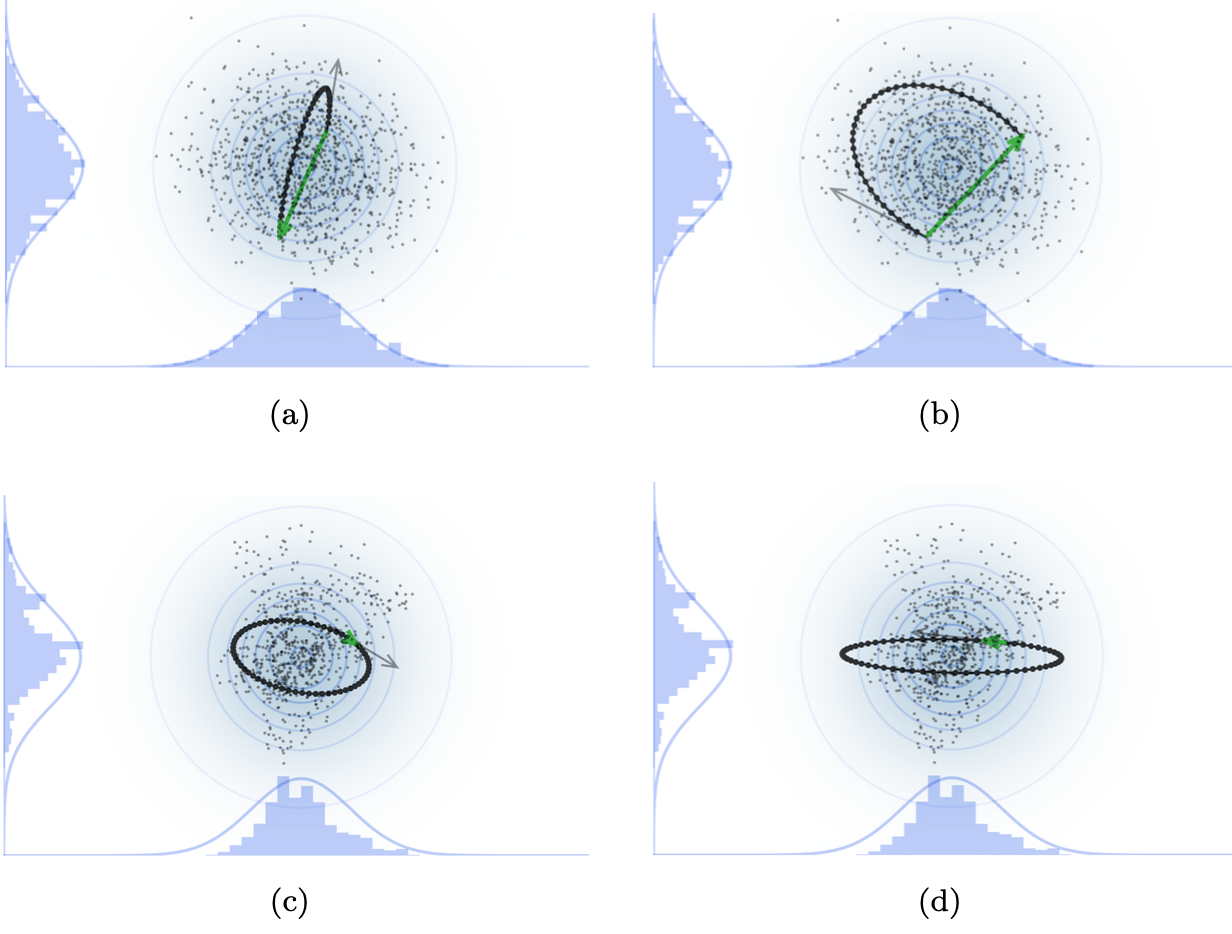
\includegraphics[width=\textwidth]{pics/HMC_Example.png}
    \caption{A simulation example with HMC for a bivariate Gaussian target distribution with $\boldsymbol{\mu}= \begin{bmatrix}
            0 & 0
            \end{bmatrix}$ and covariance matrix
            $\boldsymbol{\Sigma}= 
            \begin{bmatrix}
                1 & 0\\
                0 & 1   
            \end{bmatrix}$. Subfigure (a) and (b) shows a HMC simulation example with a proper choice for $\varepsilon$ and $L$, where the target distribution is thoroughly explored. Subfigure (c) and (d) is the same example, modified with a poor choice of values for $\varepsilon$ and $L$, where the target distribution is poorly approximated. This is especially clear on the plots of the marginal distributions where the histograms are far from the plotted correct distribution. The result is the U-Turn effect, which yield an ineffective exploration of the target distribution. The example has been generated with the interactive gallery provided by \cite{feng} \textcopyright MIT.}
    \label{fig:HMC_Example}
\end{figure}


\subsection{No-U-Turn Hamiltonian Monte Carlo}
In this section we present an algorithm introduced by \cite{hoffman2011nouturn} and evaluated by \cite{nishio_arakawa_nouturn} whose explanation we found more clear and concise. NUTS extends HMC by eliminating the need to specify the trajectory length $L$. This algorithm goes under the name No-U-Turn (NUTS) as it avoids the possible U-Turning behavior shown in figure \ref{fig:HMC_Example} (c) and (d). This is done by introducing a criterion that tells us when to stop simulating the dynamics to prevent a possible U-turn. The authors defines this criterion to be when more iterations will no longer increase the distance between the proposed state $\boldsymbol{\theta}^{\text{cand}}$ and the the initial value $\boldsymbol{\theta}^{(0)}$. More specifically, they choose a criteria, based on the derivative with respect to time of half the squared distance between the initial parameter $\boldsymbol{\theta}^{(0)}$ and the current state $\boldsymbol{\theta}^{\text{cand}}$, meaning the leapfrog steps are run until. 
\begin{equation*}
\begin{split}
    \frac{d}{d t} \frac{(\boldsymbol{\theta}^{\text{cand}}-\boldsymbol{\theta})^\top \cdot(\boldsymbol{\theta}^{\text{cand}}-\boldsymbol{\theta})}{2}&=(\boldsymbol{\theta}^{\text{cand}}-\boldsymbol{\theta})^\top \cdot \frac{d}{d t}(\boldsymbol{\theta}^{\text{cand}}-\boldsymbol{\theta})\\
    &=(\boldsymbol{\theta}^{\text{cand}}-\boldsymbol{\theta})^\top \cdot \boldsymbol{\rho}^{\text{cand}} < 0
\end{split}
\end{equation*}
However \cite{hoffman2011nouturn} notes that by doing this does we do not have the guarantee of time reversibility, so the sampling algorithm might not converge to the correct distribution. NUTS overcomes this problem by using slice sampling and applying a double method suggested by \cite{neal_slice_sampling}. 
\\
\\
NUTS augments the the model of HMC $p \lr{\boldsymbol{\theta}, \boldsymbol{\rho}} \propto \exp{\left(\mathcal{L} \lr{\boldsymbol{\theta}} - \frac{1}{2} \boldsymbol{\rho} \cdot \boldsymbol{\rho}\right)}$ to include a slice variable $u$ so that the joint probability of $\boldsymbol{\theta}, \boldsymbol{\rho}$ and $u$ is 
\begin{equation*}
    p \lr{\boldsymbol{\theta}, \boldsymbol{\rho}, u} \propto \mathbf{1} \lrs{ u \in \lrs{0,\exp{\left(\mathcal{L} \lr{\boldsymbol{\theta}} - \frac{1}{2} \boldsymbol{\rho}^\top \boldsymbol{\rho}\right)}}}
\end{equation*}
meaning that the unnormalized marginal probability of $\boldsymbol{\theta}$ and $\boldsymbol{\rho}$ (gained by integrating over $u$) is 
\begin{equation*}
    p \lr{\boldsymbol{\theta}, \boldsymbol{\rho}} \propto \exp{\left(\mathcal{L} \lr{\boldsymbol{\theta}} - \frac{1}{2} \boldsymbol{\rho}^\top \boldsymbol{\rho}\right)}
\end{equation*}
as in standard HMC. The conditional probabilities $p \lr{u \mid \boldsymbol{\theta}, \boldsymbol{\rho}}$ and $p \lr{\boldsymbol{\theta}, \boldsymbol{\rho} \mid u}$ are each uniform as long as the condition 
\begin{equation} \label{eq:nuts_unif_condition}
    u \leq \exp{\left(\mathcal{L} \lr{\boldsymbol{\theta}} - \frac{1}{2} \boldsymbol{\rho}^\top \boldsymbol{\rho}\right)}
\end{equation}
is satisfied. The challenge of slice sampling is to find the bounds the region for which this condition is satisfied. \cite{neal_slice_sampling} proposes a doubling method, where the size of the an initial segment containing the current value of $\boldsymbol{\theta}$ is randomly chosen while the segment is expanded by doubling its size until the points are outside of the region. The expanding directions are randomly chosen to be leapfrog steps forward or backward in the Markov chain to satisfy reversibility.
\\
\\
NUTS generates a finite set of all $\lr{\boldsymbol{\theta}, \boldsymbol{\rho}}$ by iteratively doubling its size. The doubling process is stopped to satisfy the condition 
\begin{equation*}
    \lr{\boldsymbol{\theta}^+ - \boldsymbol{\theta}^-}^\top \boldsymbol{\rho}^- < 0 \quad \text{or} \quad \lr{\boldsymbol{\theta}^- - \boldsymbol{\theta}^+}^\top \boldsymbol{\rho}^+ < 0
\end{equation*}
where $\boldsymbol{\theta}^+, \boldsymbol{\rho}^-$ and $\boldsymbol{\theta}^+, \boldsymbol{\rho}^-$ is the leftmost and rightmost variables of all $\lr{\boldsymbol{\theta}, \boldsymbol{\rho}}$ generated by the doubling process respectively. 
\\
\\
A subset of proposal candidates $\lr{\boldsymbol{\theta}, \boldsymbol{\rho}}$, denoted by $\mathbb{C}$, is selected from the doubling process to satisfy the condition in equation \ref{eq:nuts_unif_condition}. The new values of $\lr{\boldsymbol{\theta}^*, \boldsymbol{\rho}}^*$ are then afterward sampled uniformly from $\mathbb{C}$. 
\\
\\
To further improve this algorithm \cite{hoffman2011nouturn} used the following transition kernel in each step of doubling
\begin{equation*}
\footnotesize
T\left(\boldsymbol{\theta}^{*}, \boldsymbol{\rho}^{*} \mid \boldsymbol{\theta},\boldsymbol{\rho}, \mathbb{C}\right)=\begin{cases} \frac{\mathbf{1}\left[\boldsymbol{\theta}^{*}, \boldsymbol{\rho}^{*} \in \mathbb{C}^{\text{new}}\right]}{\left|\mathbb{C}^{\text{new}}\right|} & \text{  when } \left|\mathbb{C}^{\text{new}}\right|>\left|\mathbb{C}^{\text{old}}\right|\\
\frac{\left|\mathbb{C}^{\text{new}}\right|}{\left|\mathbb{C}^{\text{old}}\right|} \frac{\mathbf{1}\left[\boldsymbol{\theta}^{*}, \boldsymbol{\rho}^{*} \in \mathbb{C}^{\text{new}}\right]}{\left|\mathbb{C}^{\text{new}}\right|}+\left(1-\frac{\left|\mathbb{C}^{\text{new}}\right|}{\left|\mathbb{C}^{\text{old}}\right|}\right) \mathbf{1}\left[\left(\boldsymbol{\theta}^{*}, \boldsymbol{\rho}^{*}\right)=(\boldsymbol{\theta}, \boldsymbol{\rho})\right] 
&\text{  when } \left|\mathbb{C}^{\text{new}}\right|\leq\left|\mathbb{C}^{\text{old}}\right|
\end{cases}
\end{equation*}
where $\mathbb{C}^{\text{new}}$ is the subset of $\lr{\boldsymbol{\theta}, \boldsymbol{\rho}}$, denoted by $\mathbb{C}$ added by the last step of doubling and $\mathbb{C}^{\text{old}}$ is the disjoint subset of $\mathbb{C}$ so that $\mathbb{C} = \mathbb{C}^{\text{new}} \cup \mathbb{C}^{\text{old}}$ and $\lr{\boldsymbol{\theta}, \boldsymbol{\rho}} \in \mathbb{C}^{\text{old}}$. This transition kernel proposes a move from $\mathbb{C}^{\text{old}}$ to a random state $\mathbb{C}^{\text{new}}$ and accepts this move with probability $\frac{\mathbb{C}^{\text{new}}}{\mathbb{C}^{\text{old}}}$. The authors show that $T$ satisfies the detailed balance condition so that it leaves the uniform distribution over $\mathbb{C}$ invariant. According to \cite{nishio_arakawa_nouturn} this transitional kernel permits memory-efficient implementation and produces larger jumps on average than simple uniform sampling. 
\\
\\
NUTS is especially efficient as it can automatically choose a step size that achieves an acceptance probability around a desired level. The stepsize $\varepsilon$ for the $j$th iteration of a NUTS Markov chain is tuned as follows
\begin{equation*}
    \begin{split}
        \log\lr{\varepsilon_{j+1}} &\leftarrow \mu - \frac{\sqrt{j}}{\gamma} \frac{1}{j + j_0} \sum_{i=1}^j \lr{\delta - \alpha_j}\\
        \log \lr{\bar{\varepsilon}_{j+1}} &\leftarrow \eta_j \log \lr{\varepsilon_{j+1}} + \lr{1 - \eta_j} \log \lr{\bar{\varepsilon}_j} \\
        \varepsilon_{j+1} &\leftarrow \bar{\varepsilon}_{j+1}
    \end{split}
\end{equation*}
where $\alpha_j$ is an actual acceptance probability for the $j$th iteration, $\delta$ is the desired average aceptance probability, $\mu$ is a freely chosen point that the iterated $\varepsilon_j$ shrink towards, $\gamma$ is a free parameter that controls the shrinkage amount towards $\mu$ and $j_0$ is a free parameter that dampens early exploration. 
\\
\\
\cite{hoffman2011nouturn} introduces the variables $\eta_j = j^{-\kappa}$ with $\kappa < 1$ to give more recent iterates more weight. They recommend setting $\mu = \log \lr{10 \varepsilon_1}$ and $\delta \approx 0.6$, it is unclear if this is general or for logistic regression, which is what they work with in the article. They show that this way of adapting stepsize guarantees that $\alpha \rightarrow \delta$.
\\
\\
NUTS tunes $\varepsilon$ during a predetermined warm-up phase and fixes this value thereafter. Since the algorithm accepts or rejects $\lr{\boldsymbol{\theta}^*, \boldsymbol{\rho}^*}$ from multiple candidates, an alternative statistic to the Metropolis acceptance probability must be defined. They do this by defining for each iteration the acceptance probability by
\begin{equation*}
    \alpha_{j}=\frac{1}{\left|B_{j}\right|} \sum_{\boldsymbol{\theta}, \boldsymbol{\rho} \in B_{j}} \min \left\{1, \frac{p\left(\boldsymbol{\theta}^{j}, \boldsymbol{\rho}^{j}\right)}{p\left(\boldsymbol{\theta}^{j-1}, \boldsymbol{\rho}^{j, 0}\right)}\right\}
\end{equation*}

\begin{algorithm} \label{alg:nuts}
    \SetAlgoLined
    \KwInput{$\boldsymbol{\theta}^{(0)}, \varepsilon \text { and values of } \delta, \mu, \gamma, j_{0}, \boldsymbol{\kappa}, J, J^{\text{adapt}}$}
    \KwOutput{Samples from the target distribution}
    \For{j=1 to J}{
    Sample momentum $\boldsymbol{\rho}^{\text{init}} \sim N(0, \mathit{I})$\\
    Sample auxiliary variable $u \sim \operatorname{Uniform}\left(0, \exp \left(\mathcal{L}\left(\boldsymbol{\theta}\right)-\frac{1}{2}\boldsymbol{\rho}^{\text{init}^{\top}} \mathit{I}^{-1} \boldsymbol{\rho}^{\text{init}}\right)\right)$\\
    Generate $\mathbb{C}$ by using the doubling method with transition kernel $T$. \\
    Compute acceptance probability: $\alpha_{j}=\frac{1}{\left|B_{j}\right|} \sum_{\theta, \boldsymbol{\rho} \in B_{j}} \min \left\{1, \frac{p\left(\boldsymbol{\theta}^{j}, \boldsymbol{\rho}^{j}\right)}{p\left(\boldsymbol{\theta}^{j-1}, \boldsymbol{\rho}^{\text{init}}\right)}\right\}$\\
     Accept the proposal $\left(\boldsymbol{\theta}^{*}, \boldsymbol{\rho}^{*}\right)$ with probability $\alpha_{j}$. \\
    \uIf{$j\leq J^{\text{adapt}}$}{
    Update $\varepsilon_{j}$ by dual averaging. }
    \Else{
    $\varepsilon_{j}=\varepsilon_{J^{\text{adapt}}}$
    }    
    }
     \caption{No-U-Turn Sampler with Dual Averaging. For a more detailed pseudocode see \cite{hoffman2011nouturn}.}
\end{algorithm}





\section{Priors}\label{sec:priors}
From section \ref{sec:bayesian_stat} and the example given in section \ref{sec:simple_BNN} it is seen that Bayesian inference starts with a prior for the model parameters, which is suppose to embody ones prior beliefs about the assigned task. The prior is an important component and choosing a bad prior can greatly affect the resulting posterior. That said, the prior does have a diminishing effect on the posterior as the number of samples grow, as the likelihood will concentrate the posterior around a few highly likely parameters, but the effect of the prior persists even though it can be so small, that one can miss it computationally, and this might take a lot of data. One might think that if one has no qualified prior belief, then a weak prior, like a wide uniform distribution, can be a safe bet. This can however have unforeseen consequences as pointed out by \cite{lemoine2019} and \cite{sarma_kay2020}. \\
\\
The prior component is however more than a dangerous element that threatens the quality of the posterior. The prior provides a principled mechanism for researchers to incorporate previous research and knowledge into the model. Priors can also be beneficial in small samples sizes as the prior acts to regularize and reduce the chances of overfitting.
However in neural networks the relationship between parameters and the problem can be very abstract and not as intuitive as in other machine learning models like linear regression models or SVMs, so having qualified prior beliefs about the network might not be so easy. \\
\\
\cite{neal2012bayesian} stresses that even though it can seem like BNNs can be threatened by a lack of a suitable prior this is not the case, as much past work shows useful criteria for selecting suitable priors, even without full understanding of what the prior over the parameters will mean in terms of the output of the network. \cite{mackay1991} and \cite{MacKay1992} has produced results, that Neal describes as at least reasonable, by giving the parameters Gaussian prior distributions. He lets the variance of these distribution be selected as a hyperparameter, which allows the model to adapt to the data. In his work MacKay emphasizes the advantage of this approach along with hierarchical models described in section \ref{sec:hier_models}.\\
\\
\cite{buntine_weigend1991} discuss several schemes for choosing priors which favour neural networks that produce either high or low accuracy on individual examples, which in regression corresponds to expecting the variance to be certain amount, or compute smooth functions, with smoothness indicating how much predictions vary as the network inputs are changed. The degree of preference is then controlled by a hyperparameter. In this way they link the choice of prior for the network-parameters to the actual effect on these parameters on the network-function, which is clearly necessary for priors to represent beliefs about the function. 
\\
\\
In a BNN the role of the hyperparameters for the priors of the parameters correspond roughly to he role of the weight decay constant $\alpha$ in equation \ref{eq:reg_obj_func} used in training of a conventional neural network. But as noted by \cite{neal2012bayesian} these hyperparameters in BNNs can be found without the need for a validation set.


\subsection{Hierarchical Models} \label{sec:hier_models}
According to \cite{neal2012bayesian}, our prior knowledge will often be too unspecific to fix the parameter values chosen for the prior distribution, even if we have complete insight into their effects on the prior. We may then wish to treat these values as unknown hyperparameters, giving them a higher-level broad prior distribution, which we call a hyper-prior. This is what Neal calls Hierarchical models. \\
\\
One benefit of such models is appropriate degree of regularization for the task can be determined automatically from the data (\cite{mackay1991} and \cite{MacKay1992}). By allowing the parameters of the prior to be set by the data, we let the data determine the scale.\\
\\
The literature on the choice of priors and hyper-priors in hierarchical models is vast and often focused on certain applications. As it does not add to our general presentation of Bayesian neural networks or the evaluations in chapter \ref{chap:eval_NN} we will not pursue this topic further, but one can read more about this in \cite{gelmanbda04}.





% \section{Variational Inference Methods}
% In the purpose of approximating a posterior distribution,  Variational inference (VI) is an alternative to MCMC methods, for taking a fully Bayesian approach when we have complex posterior distribution which is difficult to evaluate directly or generate samples from. Whereas MCMC techniques, provide a numerical approximation, VI provides a locally-optimal solution to an approximation of the posterior, thus VI turns approximate posterior inference into an optimization problem (\cite{VI}). We consider a family of approximating densities of the model parameters $q(\boldsymbol{\theta} ; \boldsymbol{\phi})$, parameterized by $\boldsymbol{\phi} \in \boldsymbol{\Phi}$.VI finds the parameters that minimize the KL divergence from equation \ref{eq: KL} to the posterior,
% $$
% \boldsymbol{\phi}^{*}=\underset{\phi \in \boldsymbol{\Phi}}{\arg \min } \mathrm{KL}(q(\boldsymbol{\theta} ; \boldsymbol{\phi}) \| p(\boldsymbol{\theta} \mid \boldsymbol{x})) .
% $$
% The optimized $q(\boldsymbol{\theta};\boldsymbol{\phi}^{*})$ is then an approximation of the posterior distribution. This is often not computable, since it requires that we are able to calculate the evidence $\ln p(\boldsymbol{X})$ which we often are not able to. Instead we maxmise the Evidence lower bound (ELBO)
% \begin{equation*}
%     \mathscr{L}(\boldsymbol{\phi})=\mathbb{E}_{q(\boldsymbol{\theta})}[\log p(\boldsymbol{x}, \boldsymbol{\theta})]-\mathbb{E}_{q(\boldsymbol{\theta})}[\log q(\boldsymbol{\theta} ; \boldsymbol{\phi})]
% \end{equation*}
% We note that the E


% \subsection{Automatic Variational Inference}\label{sec:ADVI}
% \subsection{Bayes by Backprop}
% \textcolor{red}{Maybe this section should be something we could mention as for future work? as the PYMC VI implementation is build on ADVI (\ref{sec:ADVI}) and not Bayes by Backprop? Otherwise we should check if we can build this our selfs? I have not yet seen it implemented.}
